\chapter{Implementation of Pipelined Maritime Surveillance and Teacking System}

The process of turning a carefully drafted system design into a working real-time surveillance pipeline requires careful attention to the integration of the different tools, frameworks, and data flows for each processing stage. The proposed maritime surveillance system integrates the entirety of the design choices made in the previous chapter, and extends them to become a fully functional system that can be tested.The proposed maritime surveillance system combines the entire design decisions that were made in the previous chapter, extends this and makes them operational and viewable in a system that can be tested. Each module was designed, configured and tested separately before being integrated into the complete end-to-end system to make sure that any errors could be detected and corrected at the module level before the integration of the entire system was made. The chapter provides a detailed description of the system implementation in practice, which includes the development environment, dataset preparation procedures, model training configurations, implementation specifics for each module, and the strategies used to obtain a stable real-time throughput, and hence, a complete and reproducible account of the realisation of the proposed design. Below is the pipeline architecture of the proposed system.

\begin{figure}[htb]
\centering
	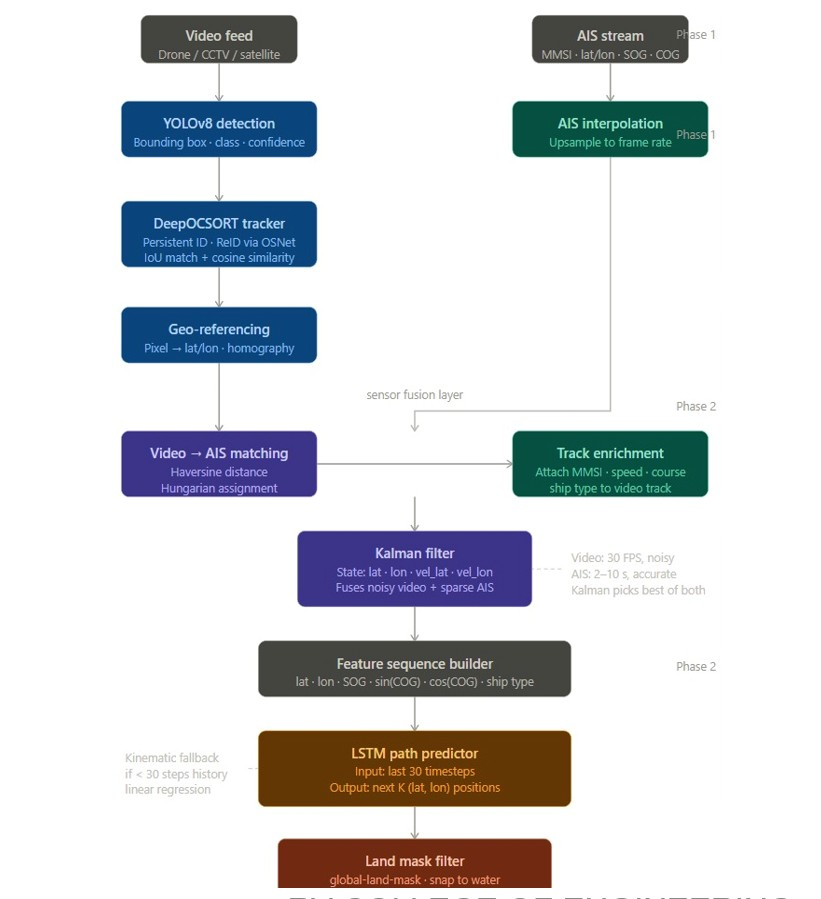
\includegraphics[scale=1]{Chapter4/Figures/pipeline.jpeg}	
	\caption{Pipeline of the proposed system }
	\label{fig:universe}
\end{figure}


\section[Top-Level System Design and Implementation]{\textbf{Top-Level System Design and Implementation}}

The proposed maritime surveillance system is a fully software-based implementation built upon a modular pipeline architecture. The top-level design integrates six primary functional modules — video ingestion, ship detection, multi-object tracking, sensor fusion, trajectory prediction, and geospatial visualisation — each implemented as an independent unit that communicates with adjacent stages through well-defined data interfaces. The following sections elaborate the implementation details of each module.

\subsection{\textbf{Development Environment and Configuration}}
The system is implemented in Python 3.8, with PyTorch serving as the primary deep learning framework for both the YOLOv8 detection model and the LSTM trajectory predictor. OpenCV handles all video ingestion, frame extraction, and real-time annotation rendering. NumPy and Pandas manage intermediate data structures including bounding box arrays, centroid coordinate histories, and trajectory sequence buffers. Matplotlib provides offline visualisation of tracking outputs and predicted paths, while Folium renders interactive geospatial maps displaying vessel positions in real-world latitude-longitude coordinates. The entire pipeline is executed on an NVIDIA GPU-enabled environment with CUDA acceleration, ensuring that frame-level processing meets the 30 FPS real-time throughput requirement. Development and testing were conducted using Jupyter Notebook and VS Code as the primary integrated development environments.

\subsection{\textbf{Dataset Preparation and Annotation}}
Maritime video datasets were sourced and preprocessed to generate the training corpus for the YOLOv8 detection model. Raw video footage was segmented into individual frames at uniform sampling intervals, producing a diverse image dataset encompassing varied sea states, vessel types, illumination conditions, and occlusion scenarios. Each frame was annotated using bounding box labels in YOLO format, with each annotation specifying the class identifier and normalised centre coordinates, width, and height of every vessel instance present. The annotated dataset was partitioned into training, validation, and test splits following a 70:20:10 ratio. Data augmentation techniques — including horizontal flipping, brightness and contrast jittering, random cropping, and mosaic augmentation — were applied during training to improve model generalisation and robustness across unseen maritime conditions.

The Top-Level System Design and Implementation section outlines the overall design and implementation of the system at a high level.The Top-Level System Design and Implementation section describes the overall design and implementation of the system at a high level.

The proposed maritime surveillance system is a fully software-based system, based on a modular pipeline architecture. The high-level design consists of six main functional modules – video ingestion, ship detection, multi-object tracking, sensor fusion, trajectory prediction, and geospatial visualisation – with each module being a standalone entity that provides clearly defined data interfaces to connect with neighbouring modules. The next sections discuss the details of the implementation of each module.

Subsection Development Environment and Configuration
The entire system is developed in python 3.8, and PyTorch is used as the main deep learning framework for the detection model (YOLOv8) and trajectory predictor (LSTM). OpenCV provides functionality to ingest all video footage, extract frames and render all the annotations in real time. Intermediate data structures such as bounding box arrays, centroid coordinate histories, and trajectory sequence buffers managed by NumPy and Pandas. Matplotlib allows for plotting tracking outputs and predicted tracks offline, and Folium generates interactive geospatial mapping with customizable features for plotting vessel positions in world coordinates (latitude and longitude). The whole pipeline is implemented in an NVIDIA GPU accelerated environment, CUDA, that guarantees the real-time throughput of 30 FPS at the frame level. The primary integrated development environment used for development and testing were Jupyter Notebook and VS Code.

\subsection{Data Collection and Data Annotation}
All the maritime video data were collected and pre-processed to create the training data set for the YOLOv8 detection model. The raw video data was then partitioned into individual frames with a fixed sampling interval, resulting in a wide range of images representing varying sea-states, vessel types, illumination conditions and occlusion scenarios. The images were annotated using bounding box labels in YOLO format that included the class identifier and normalised centre coordinates, width and height of all the vessels instances within each image. The data set was divided into training, validation, and test sets, with ratios set as 70:20:10. To enhance the generalisation and robustness of the model for unseen maritime conditions, data augmentation techniques were used during training, such as horizontal flipping, brightness and contrast jittering, random cropping and mosaic augmentation.

The Ship Detection Module is YOLOv8.YOLOv8 is Ship Detection Module.
Pretrained COCO weights were used to initialise the YOLOv8 model and the model was fine-tuned with the prepared maritime dataset using transfer learning. The training was done with the Stochastic Gradient Descent (SGD) optimiser, the Cosine Annealing learning rate scheduler and early stopping based on the convergence of the validation mAP. The model has been configured to have a confidence threshold of 0.5 and an IoU threshold of 0.45 for Non-Maximum Suppression during inference. During runtime, for every video frame extracted, it is input into the trained YOLOv8 model that outputs a list of bounding box predictions, confidence scores, and class labels for all the detected vessels. Any detections that are not above the confidence level will be ignored and not sent to the tracking module.

The Multi-Object Tracking Module — DeepOCSORT module is used to track the objects in the image.The Multi-Object Tracking Module — DeepOCSORT module is applied to track objects in the image.
Confirmed detections by the YOLOv8 module are fed to the DeepOCSORT tracker, which is initialised with a maximum track age of 30 frames, a minimum hit count of 3 for the tracker to be considered as a confirmed track, and cosine similarity metric for Re-Identification (RI). OSNet is used as the appearance embedding extractor and results in compact feature vectors of detected vessels, which are encoding appearance identity information without position information. DeepOCSORT first matches detections to track predictions at every frame according to IoU, and then further matches the detections to the track predictions by cosine similarity using ReID embeddings in order to disambiguate the matching. Successful matches update the corresponding tracks, unmatched detections start new tentative tracks and tracks that do not get a match within the maximum age are removed. The coordinates of all tracks that have been determined as active at each frame are extracted and stored in a moving track buffer for use in downstream motion analysis and prediction.

\subsection{\textbf{Motion Parameter Estimation}}
The tracking module stores a history of the centroid coordinates, which is used to compute inter-frame motion parameters analytically. Instantaneous vessel speed is computed as the Euclidean distance travelled per unit time between the centroid of neighbouring frames, for each active track. The heading angle is found by taking the arctangent of the vertical and horizontal displacement components and the cardinal direction (North, South, East, West and their intermediate directions) is produced by dividing the calculated heading angle into direction bins. These motion parameters are added to the video output stream together with the Bounding Boxes and the Tracking ID's, so that the operator is given a live stream of the motion parameters for each tracked vessel.

Finally, the sensor fusion – AIS integration and Kalman filter are discussed.
AIS data (with MMSI identifiers, latitude, longitude, Speed Over Ground (SOG) and Course Over Ground (COG)) is received concurrently with the video data and upsampled using linear interpolation to the video frame rate. The positions of video track are geo-referenced by applying a pre-computed homographic transformation matrix to the video centroid pixel positions, and the matched AIS records are found through Haversine distance computation and Hungarian assignment algorithm. tracks that are successfully matched will be enhanced with AIS vessel attributes. A Kalman filter is then applied to the fused state, with the state vector containing latitude, longitude and velocity in the latitude and longitude directions. The Kalman filter prediction and update steps combine the high-frequency video observations, which are noisy and uncertain, with the limited (but high accuracy) AIS observations, to get a smooth and stable estimate of each vessel's geographic position at each timestep.

\subsection{\textbf{Trajectory Prediction Module — LSTM}}
The LSTM is used to predict the trajectory in the Trajectory Prediction Module.In the Trajectory Prediction Module the LSTM is used to predict the trajectory.
The LSTM trajectory predictor is a sequential neural network, consisting of two stacked LSTM layers and a fully connected output layer. The model is trained on input sequences of data of length 30 timesteps, each timestep being a feature vector composed of latitude, longitude, SOG, sin(COG), cos(COG) and ship type encoding data. The network was trained on historical track data using a loss function known as Mean Squared Error (MSE) and the Adam optimiser. During the runtime the feature sequence builder constructs the 30-step window for the input data, from the history of the track of the Kalman-filtered vessels, and passes it to the trained LSTM model, which returns the predicted geographic coordinates for the next K positions of the vessels. To achieve this, the kinematic linear regression fallback is automatically enabled for tracks with less than 30 timesteps of history, allowing for track output whether or not the track is new.

\subsection{\textbf{Land Mask Filter and Geospatial Visualisation}}
The predicted trajectory coordinates are sent to a Land mask filter which compares each predicted point with a global land-water mask to check if it is either in land or water. Predictions that fall on land areas that are indicative of physically unrealistic vessel routes due to prediction uncertainty are snapped to the nearest valid water coordinate to limit all predictions to operationally realistic maritime areas. Detection bounding boxes, unique tracking ID, motion-parameter annotations, historical trajectory overlay and predicted path markers are drawn on the live video stream by OpenCV. At the same time, the positions of vessels and potential paths are displayed on an interactive Folium map, delivering to the boat operator a geospatial, real-time dashboard for all maritime situational awareness.
You can add sections and sub sections to elaborate your project work done.

\vspace{0.75cm}
\section{Summary}
This chapter fully implemented the proposed end-to-end maritime surveillance system, and this system was based on the architectural design developed in Chapter 3, to enable the technology to be fully operational and real-time. The development environment was defined and the technology stack consists of Python, PyTorch, OpenCV, NumPy, Pandas, Matplotlib and Folium, with the processing power and acceleration of the system provided by NVIDIA CUDA. The data preparation and data annotation process were explained, including extraction of frames from the video and labelling the YOLO format, partitioning of the data and methods used to augment the data to increase model generalisation. Then the implementation of each functional module was elaborated sequentially: from the configuration of ship detection based on YOLOv8 to the development of transfer learning training configuration; from the DeepOCSORT configuration, identity-preserving tracking based on OSNet, to the inter-frame motion parameter estimation and the ingestion of the AIS stream; from Haversine-based sensor fusion to Kalman filter state smoothing. The network architecture, training process and sequence construction of features at runtime of a LSTM trajectory prediction module were described, as well as the kinematic fallback strategy for short-history tracks. Last, the pipeline's end-to-end components, the land mask filtering system and the dual-output visualisation system (OpenCV-annotated video feeds and Folium-created interactive geospatial maps) were displayed. The implementation described in this chapter is used to implement the entire surveillance framework whose performance is assessed and analysed in the following chapter.
